\section{Electroweak Diboson Physics } 
\label{sec:EWKPheno}

At the LHC, two types of physics processes contribute to the production of di-$Z$ bosons in association with two jets $[ ZZ^*( \rightarrow 4\ell) jj ]$: the QCD production at the order $\alpha_{S}^{\geq 2} \alpha_{EWK}^{4}$ and the EWK production at order $\alpha_{EWK}^{\geq6}$ \cite{CMSRun2ZZjj}. Figures \ref{fig:ZZjjFeynmanDiag_QCD_qq} and \ref{fig:ZZjjFeynmanDiag_QCD_gg} show the Feynman diagrams at leading order for parton-initiated and gluon loop-initiated QCD $ZZ^*(\rightarrow 4\ell) jj$ processes, respectively, whereas Figure \ref{fig:ZZjjFeynmanDiag_EWk} shows the Feynman diagrams at leading order for the EWK $ZZ^*(\rightarrow 4\ell) jj$ production \cite{PowhegV2ZZjj}. The EWK production consists of two sets of interactions: the vector boson scattering processes involving either triple (Figure \ref{fig:ZZjjFeynmanDiag_EWk_a}) or quartic (Figure \ref{fig:ZZjjFeynmanDiag_EWk_b}) self-interactions of the gauge-bosons, and the processes featuring the Higgs bosons (Figure \ref{fig:ZZjjFeynmanDiag_EWk_c} and \ref{fig:ZZjjFeynmanDiag_EWk_d}). 

Figure \ref{fig:VBS_XS} shows the cross-sections as a function of the center of mass energies ($\sqrt{s}$) for the longitudinally polarized vector boson scattering, corresponding to the self-interactions of the gauge-bosons. The longitudinal cross-sections grow quadratically at high values of $\sqrt{s}$, eventually violating the unitarity bounds. The unitarity violation is observed in cross-sections for longitudinal vector boson scattering in all $V_L V_L \rightarrow V_L V_L$ processes. Figure \ref{fig:SM_XS} shows the longitudinal cross-sections for the electroweak $V_L V_L \rightarrow V_L V_L$ processes, including the amplitudes from the vector bosons self-interactions and $H\rightarrow V_L V_L$ processes. As shown, the precise interference between the Higgs-featured and VBS processes restores the unitarity at high energies for all multi-boson final states\cite {VBSWWWW}.

\begin{figure}[!htbp]
  \begin{subfigure}{.49\textwidth}
    \centering
    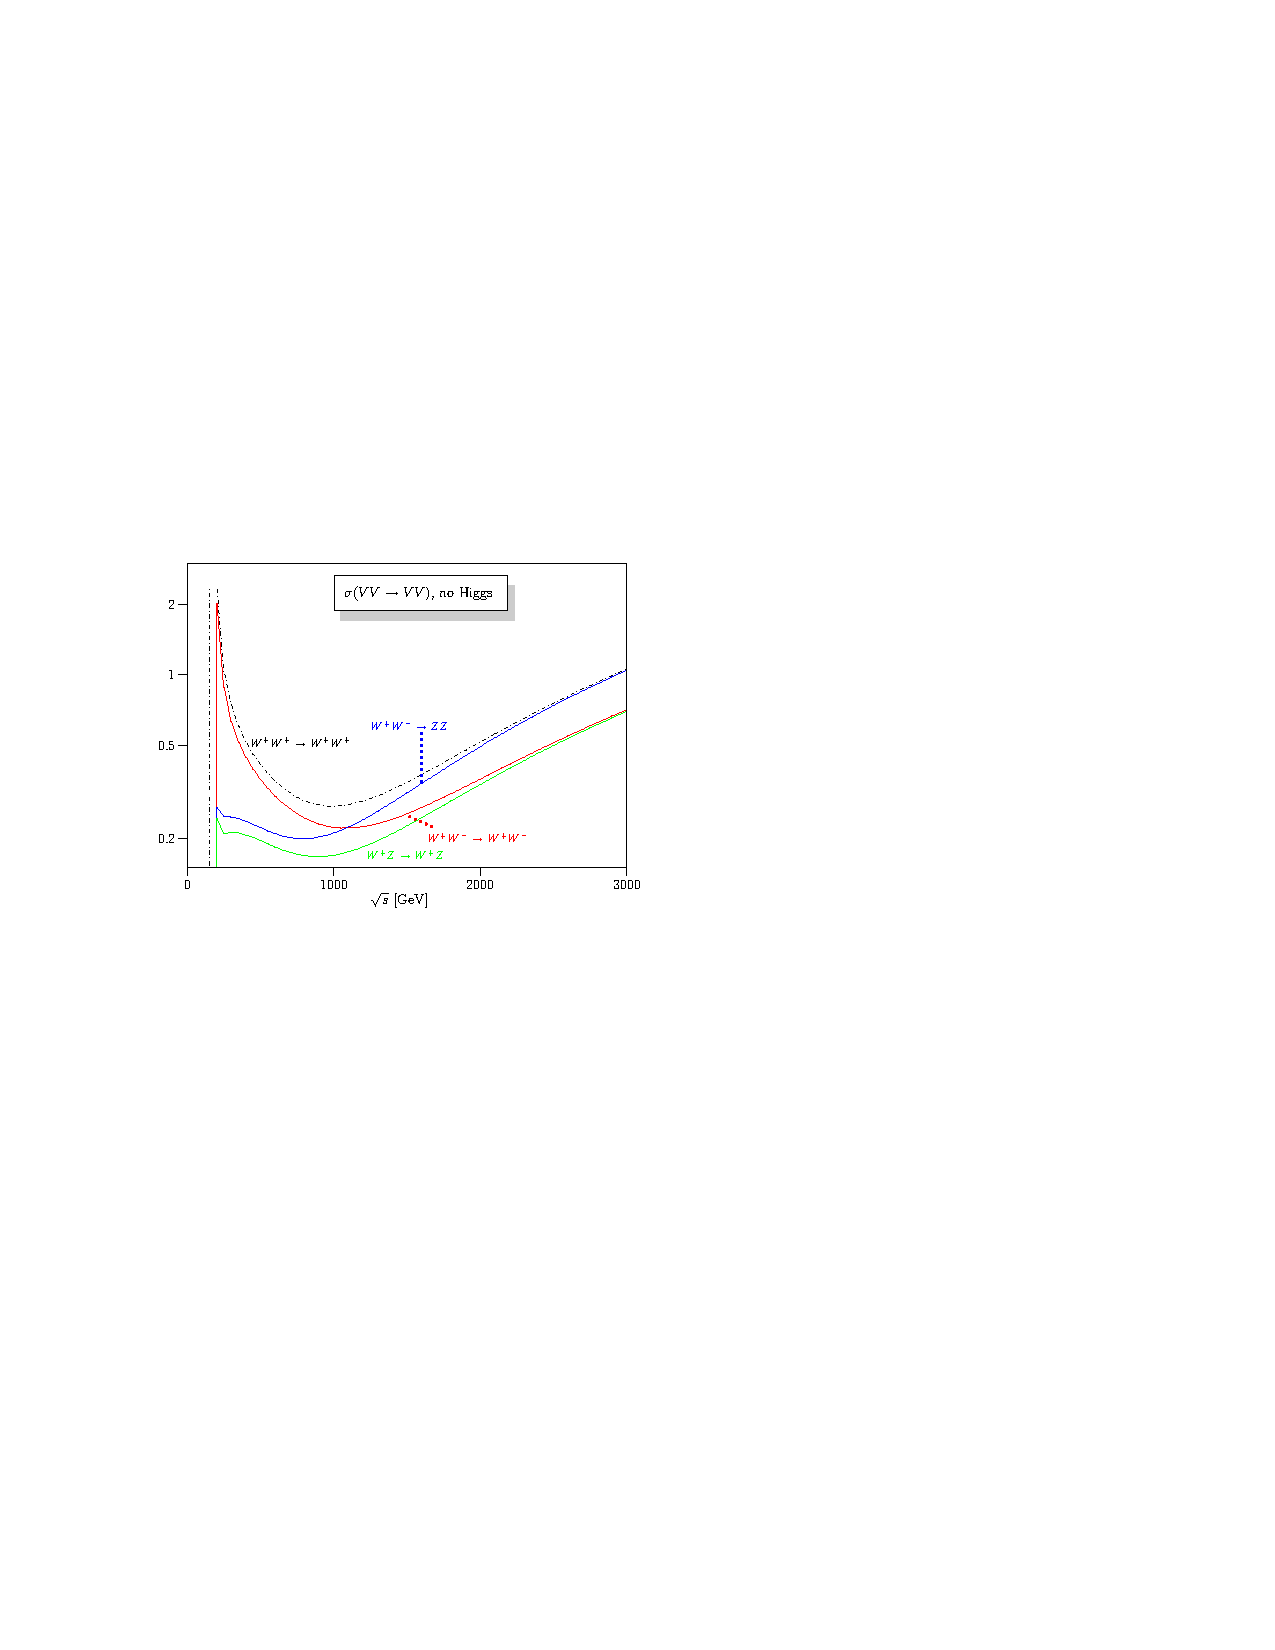
\includegraphics[width=.99\linewidth]{figures/Theory/VBS_NoHiggs.pdf}  
    \caption{$\sigma_{LL}$ for $V_L V_L \rightarrow V_L V_L$ processes.}
    \label{fig:VBS_XS}
  \end{subfigure}
  \begin{subfigure}{.49\textwidth}
    \centering
    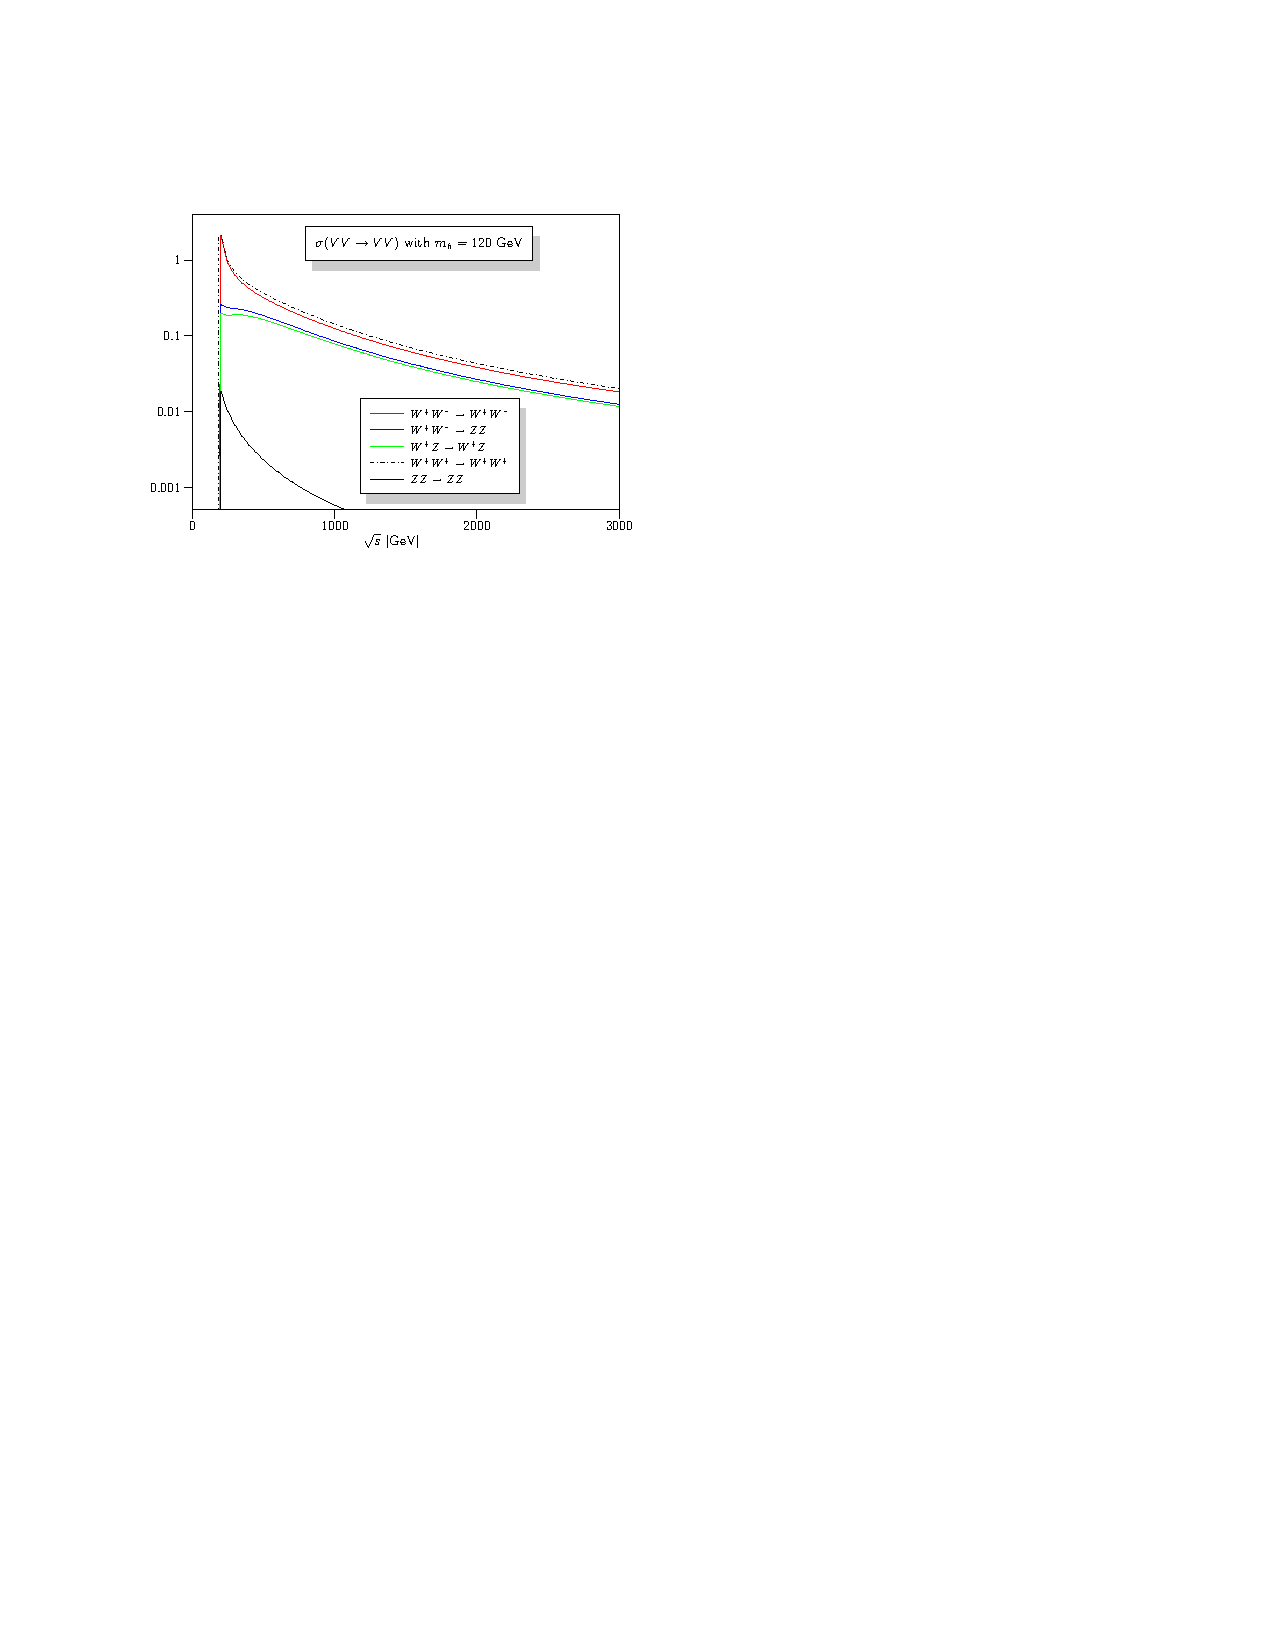
\includegraphics[width=.99\linewidth]{figures/Theory/VBS_WithHiggs.pdf}  \\
    \caption{$\sigma_{LL}$ regularization by $H\rightarrow V_L V_L$ processes.}
    \label{fig:SM_XS}
  \end{subfigure}
  \caption{ Cross-sections for longitudinal component of the electroweak $VVjj$ production as a function of $\sqrt{s}$ \label{fig:SM_EWK_ZZjj_XS} \cite{VBSDiagrams}. These calculations were made before the discovery of the SM Higgs; thus, the calculations in the second figure use an SM-like Higgs with $120$ GeV mass. For the SM Higgs with a mass of $125.10$ GeV, the regularization is similar in shape. }
\end{figure}

As discussed in Section \ref{subsubsec:HiggsMech}, the massive $W$ and $Z$ bosons get their masses via the BEH mechanism through EWSB. As a consequence of EWSB, the $W$ and $Z$ bosons acquire an additional degree of freedom (the longitudinal polarization mode) whose scattering interfere with the Higgs-featured processes. Thus, measuring the cross-sections of electroweak production of the di-$Z$ bosons in association with two jets provides a direct probe of the EWSB, which is at the heart of the SM \cite{CMSRun2ZZjj}. As the unitarity is restored at high energies, the cross-section of the electroweak $ZZ^*(\rightarrow 4\ell) jj$ process is sensitive to possible BSM modifications at high energies. Therefore, measuring the cross-sections of the electroweak $ZZ^*(\rightarrow 4\ell) jj$ processes differentially as a function of kinematically sensitive observables is essential. 

\begin{figure}[!htbp]
  \begin{center}
  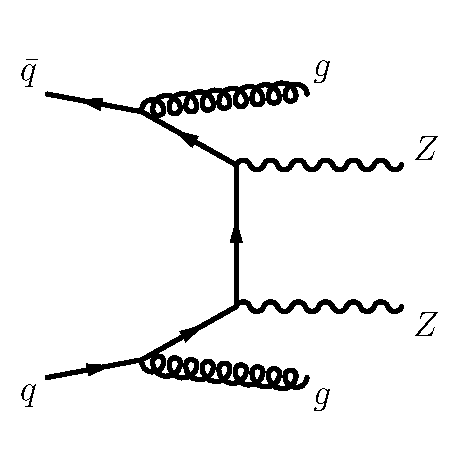
\includegraphics[width=0.31\textwidth]{figures/Theory/diagramQCDZZjjqq.pdf}
  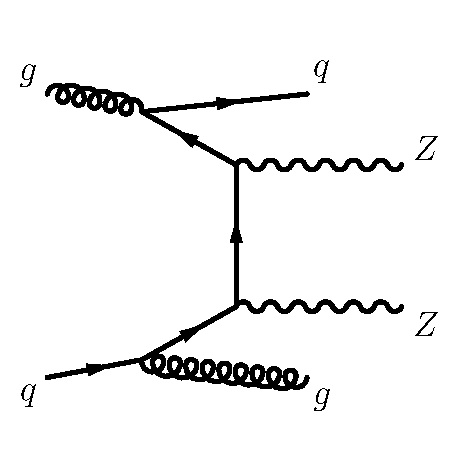
\includegraphics[width=0.31\textwidth]{figures/Theory/diagramQCDZZjjqg.pdf}
  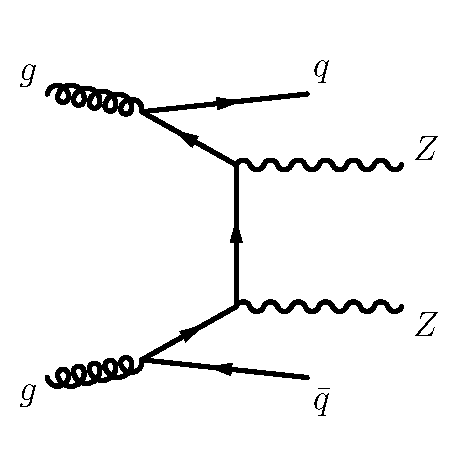
\includegraphics[width=0.31\textwidth]{figures/Theory/diagramQCDZZjjgg.pdf}
   \end{center}
  \caption{Typical diagrams of LO $qq$ and $gg$ induced QCD $\alpha_{S}^2 \alpha_{EWK}^{2}$ production of $ZZ^*jj$. The two $Z\rightarrow \ell \ell$ vertices each contribute an additional electroweak coupling of $\alpha_{EWK}$. \label{fig:ZZjjFeynmanDiag_QCD_qq}}
 \end{figure} 
 
\begin{figure}[!htbp]
  \begin{center}
  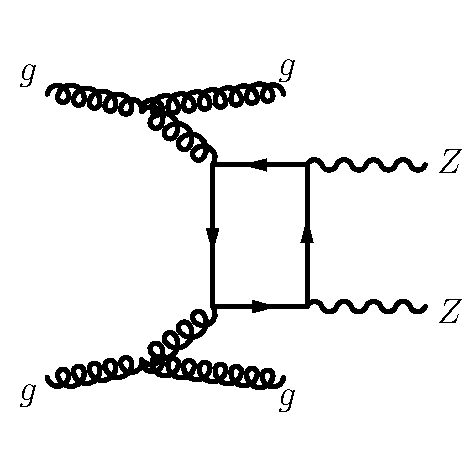
\includegraphics[width=0.31\textwidth]{figures/Theory/diagramQCDZZjjbox.pdf}
  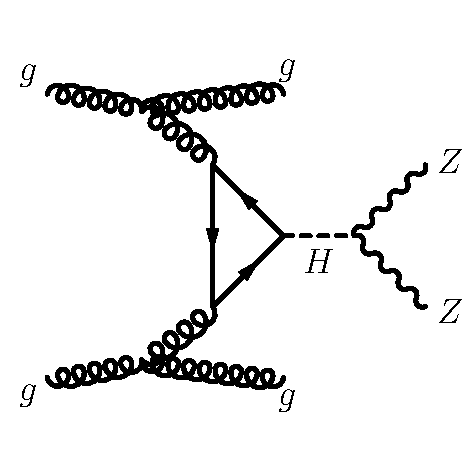
\includegraphics[width=0.31\textwidth]{figures/Theory/diagramQCDZZjjggH.pdf}\\
  \end{center}
  \caption{Typical diagrams for LO $gg$ loop induced the QCD $\alpha_{S}^4\alpha_{EWK}^{2}$ production of $ZZ^*jj$. The two $Z\rightarrow \ell \ell$ vertices each contribute an additional electroweak coupling of $\alpha_{EWK}$. \label{fig:ZZjjFeynmanDiag_QCD_gg}}
 \end{figure}
 
\begin{figure}[!htbp]
\begin{subfigure}{.49\textwidth}
  \centering
  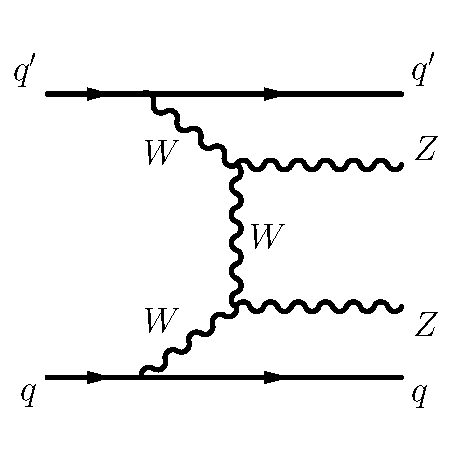
\includegraphics[width=.8\linewidth]{figures/Theory/diagramEWZZjjTGC.pdf}  
  \caption{ZZjj production with two triple gauge coupling (TGC) vertices.}
  \label{fig:ZZjjFeynmanDiag_EWk_a}
\end{subfigure}
\begin{subfigure}{.49\textwidth}
  \centering
  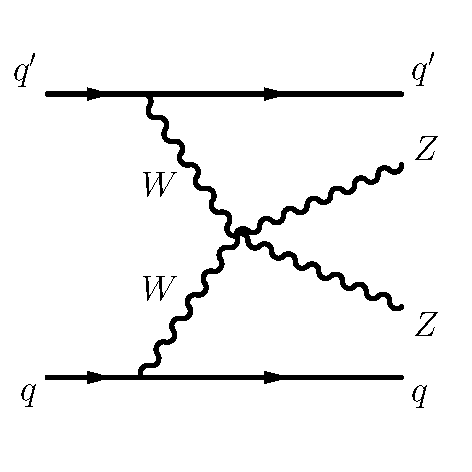
\includegraphics[width=.8\linewidth]{figures/Theory/diagramEWZZjjQGC.pdf}  \\
  \caption{ZZjj production with a quartic gauge coupling (QGC) vertex.}
  \label{fig:ZZjjFeynmanDiag_EWk_b}
\end{subfigure}
\begin{subfigure}{.49\textwidth}
  \centering
  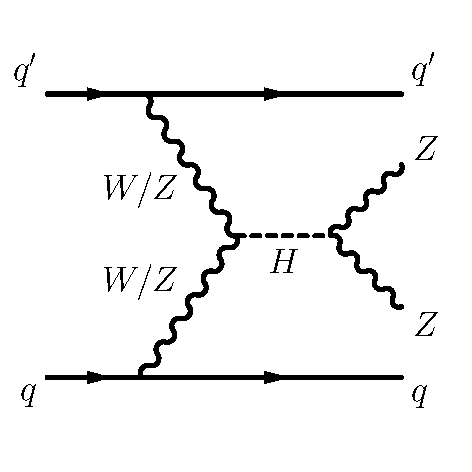
\includegraphics[width=.8\linewidth]{figures/Theory/diagramEWZZjjSchnHiggs.pdf}  
  \caption{s-channel Higgs ZZjj Production.}
  \label{fig:ZZjjFeynmanDiag_EWk_c}
\end{subfigure}
\begin{subfigure}{.49\textwidth}
  \centering
  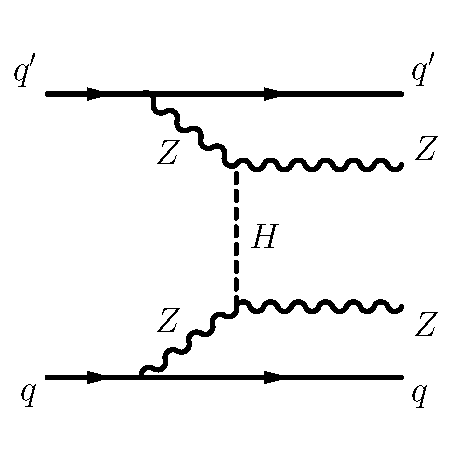
\includegraphics[width=.8\linewidth]{figures/Theory/diagramEWZZjjTchnHiggs.pdf}  
  \caption{t-channel Higgs ZZjj Production.}
  \label{fig:ZZjjFeynmanDiag_EWk_d}
\end{subfigure}\\
\caption{Feynman diagrams at LO for the EWK $\alpha_{EWK}^4$ production of $ZZ^*jj$. The two $Z\rightarrow \ell \ell$ vertices each contribute an additional electroweak coupling of $\alpha_{EWK}$. }
\label{fig:ZZjjFeynmanDiag_EWk}
\end{figure}

The triple and quartic self-interactions of the gauge bosons arise from the square of the non-Abelian structure of $SU(2)$ in the kinetic term $ \frac{1}{4} W^{a}_{\mu\nu} W^{\mu\nu}_{a}$ of the EWK Lagrangian in Equation \ref{eqn:EWKLagrangian1}. Implementing the values of the field strength tensor $W^{a}_{\mu\nu}$ from Equation \ref{eqn:SU2FST}, the relations of $W_{\mu}^{\pm}$ fields in Equation \ref{eqn:RealWBosons}, and the relations of neutral gauge fields in Equation \ref{eqn:NeutralGaugeBosons}, the triple and quartic self interaction terms become, 
\begin{equation}
\mathcal{L}_{3} = ie_{V=\gamma,Z} [ W^{+}_{\mu\nu} W^{-\mu} V^{\nu} - W^{-}_{\mu\nu} W^{+\mu} V^{\nu} + W_{\mu}^{+}W_{\nu}^{-}V^{\mu\nu} ], 
\label{eqn:L_TGC}
\end{equation}
\begin{equation}
\begin{array}{l}
\mathcal{L}_{4} = e^{2}_{W} [ W^{-}_{\mu}W^{+\mu}W^{-}_{\nu}W^{+\nu} - W^{-}_{\mu}W^{-\mu}W^{+}_{\nu}W^{+\nu} ] \\
 \hspace{10pt} + e^2_{V=\gamma,Z} [ W^{-}_{\mu}W^{+\mu}V_{\nu}V^{\nu} - W^{-}_{\mu}V^{\mu}W^{+}_{\nu}Z^{\nu} ] \\
  \hspace{10pt} + e_{\gamma}e_{Z} [ 2W^{-}_{\mu} W^{+\mu} Z_{\nu}A^{\nu} - W_{\mu}^{-}Z^{\mu}W^{+}_{\nu}A^{\nu} - W_{\mu}^{-}A^{\mu}W^{+}_{\nu}Z^{\nu} ],
\end{array}
\label{eqn:L_QGC}
\end{equation}
where $e_{\gamma} = g\sin\theta_{W}$; $e_{W} = \frac{e_{\gamma}}{2\sqrt{2}\sin\theta_{W}}$ and $e_{Z} = e_{\gamma}\cot\theta_{W}$ are the precise coupling strengths for vector boson self-interaction. Both triple and quartic neutral couplings, such as $ZZZ$ or $ZZZZ$ are absent in the SM. 

Similarly, the couplings of Higgs to vector bosons are also predicted precisely by the BEH mechanism in Equation \ref{eqn:LagBEHKin} as:
\begin{equation}
\mathcal{L}_{HVV} = \frac{m_{W}^2}{v^2} W^{+}_{\mu}W^{-\mu}h^{2} + \frac{m_{Z}^{2}}{v^2} Z_{\mu}Z^{\mu}h^{2}.
\label{eqn:HVVCoupling}
\end{equation}

The EWK production of $ZZ^*(\rightarrow 4\ell ) jj$ is extremely sensitive to any possible anomalous triple gauge couplings (aTGC), anomalous quartic gauge couplings (aQGC), or anomalous Higgs to vector boson couplings \cite{SensitivityNP} \cite{EFT_Eboli} \cite{BSM_Simple2HDM}. Therefore, it is imperative to probe the high energy behavior of the EWK production of $ZZ^*(\rightarrow 4\ell ) jj$ to seek possible deviations from the physics processes Beyond the Standard Model. 

The EWK $ZZ^*(\rightarrow 4\ell ) jj$ production with each $Z$ boson decaying to a pair of SF-OC lepton pairs is an extremely rare process. Thus, the QCD background processes dominate the $ZZ^*(\rightarrow 4\ell ) jj$ events recorded by the ATLAS detector during Run-2 \cite{ATLASZZjj}. The electroweak production of $ZZ^*jj$ shown in Figure \ref{fig:ZZjjFeynmanDiag_EWk} has some characteristic kinematic properties. In each electroweak process, the initial state quark radiates a vector boson which scatters either by self-interactions or Higgs and produces the two final state $Z$-bosons, each of which decays to the SF-OC leptons. The initial state partons continue in almost the same direction as their parent protons, forming jets on the opposite side of the ATLAS detector with a large spatial gap and no additional hadronic activity from the hard scattering between the two jets \cite{RapidityGapCite}. As the final state jets originate directly from the initial partons in the hard interaction, they are highly energetic, resulting in two jets with high momenta and a significant invariant mass\cite{RapidityGapCite}. Due to momentum conservation, the two $Z$-bosons are produced centrally with respect to the dijet. The decay of the two Z bosons into SF-OC muons or electrons defines the final signature of the VBS-$ZZ^*(\rightarrow 4\ell ) jj$-like event.

The previous ATLAS measurement of $ZZ(\rightarrow 4\ell ) jj$ used a multi-variate analysis exploiting these kinematic properties to measure the fiducial cross-sections for purely electroweak $ZZjj$ process \cite{ATLASZZjj}. Due to limited statistics in the final state, it is impossible to measure differential cross-sections for the purely electroweak $ZZ^*(\rightarrow 4\ell ) jj$ process using the LHC Run-2 dataset. Therefore, a VBS-Enhanced phase space, which includes a high fraction of events from the EWK production based on their unique kinematic properties, is defined. The differential cross-sections presented in this thesis are measured in this electroweak-enhanced phase space. 
